\documentclass[conference]{IEEEtran}
\IEEEoverridecommandlockouts
% The preceding line is only needed to identify funding in the first footnote. If that is unneeded, please comment it out.
\usepackage{cite}
\usepackage{amsmath,amssymb,amsfonts,ntheorem}
\usepackage{algorithmic}
\usepackage{graphicx,graphbox}
\usepackage{textcomp}
\usepackage{xcolor}
\usepackage{subfigure}
\usepackage{color}
\def\BibTeX{{\rm B\kern-.05em{\sc i\kern-.025em b}\kern-.08em
    T\kern-.1667em\lower.7ex\hbox{E}\kern-.125emX}}
\begin{document}

\title{Locomotion Design of \\a Bio-inspired Hexapod Robot\\}
\author{\IEEEauthorblockN{Yatian Pang}
\IEEEauthorblockA{\textit{ Department of Mechanical Engineering} \\
\textit{National University of Singapore}\\
Singapore, Singapore \\
e0576086@u.nus.edu}
}

\maketitle

\begin{abstract}
Bio-inspired robot is designed to engage in biological characteristics works, which is based on biology in nature and imitates it physiological characteristics and behavior
patterns. In this project, we explore the leg composition of insects, espeically hexapod animals, and design an flexiable hexpod robot. After analysing the gait of insects, we  design and implement a locomotion controller for the hexapod robot by solving body inverse kinematics and leg inverse kinematics. We adopt Robot Operating System to simulate body posture control and robot locomotion control. The results show that our body posture and locomotion control method is successful. Besides, our proposed contorl framework is efficent that the hexapod robot can change body postures at arbitrary time during locomotion. 

\textit{\textcolor{magenta}{Code available at: https://github.com/Pang-Yatian/hexapod}}

\textit{\textcolor{magenta}{Demo video available at: https://youtu.be/je8t2UhGXK0}}

\end{abstract}

\begin{IEEEkeywords}
Bio-inspired, hexapod, locomotion control, body posture control
\end{IEEEkeywords}

\section{Introduction}
Legged robots have been studied in recent decades in order to take advantages that demostrated by natural abilities of some animals and insects.Nevertheless, locomotion of the legged robots is quite challenging espeically when it comes to irregular terrains \cite{a2}\cite{a3}. The animals are naturally adapted to different types of surfaces. Aming to develop a similar mechanism, scientific communities are inspired and try to imitate to some extent in mechanical design, gait control etc.

One of the main challenges in the development of robots is the locomotion system design, which involves the interaction of structures composed of prismatic or rotational joints which emulates the motion functions existing in nature, allowing adapting to uneven terrain \cite{a15}. It also needs to deal with problems like the mechanical complexity existing in legs, the mechanism stability, power consumption, synchronization of the links in each of the robots joints and the control of number of degrees of freedom that is requiring.\cite{aa} In case of a hexapod robot with three degrees of freedom per leg it is required to synchronize for eighteen angles in total.

The legs location regarding the displacement surface is important in the robot’s stability, the same way as the observation of the center of gravity, owing to that if these do not have a proper synchronization and do not provide the necessary support to the system base, it will lose balance and will fall or its movements will be inefficient causing perhaps a greater energy consumption\cite{a16}. This synchronization will depend of the mobility control of the legs for its displacement, because if the robot moves withi the established limits, collisions between the links will be avoided and therefore the system will not be affected. The length and design of the legs is essential in robot locomotion, because the trajectory that is implemented in each of the articulation depend on them.

If we have the trajectory that allows a smooth movement, we will not see the robot stability affected by a hard movement and we can determine the progress of the movement in a given time. Also, if the robot moves within the established limits, the collision risk is avoided and the system will be safe.

To solve the problems mentioned above, a simulated prototype is developed in this project, with the goal to generate inspiration that learned from animals. Besides, robot locomotion controller is designed based on gait analysis of animals. We test our hexapod robot in the simulation environment and do corresponding experiments to prove the efficency of our model and controller. 

This report is arranged as follows, in section \ref{s2}, we conduct a biology analysis, in which leg composition and gait analysis will be presented. In section \ref{s3}, we will introduce the hexapod robot model design and calculate the corresponding kinematics model. In section \ref{s4}, design of the locomotion controller will be detailed. After presenting the simulation experiments in section \ref{s5}, we will conclude the whole project.

\section{Biology Analysis}\label{s2}

\subsection{Leg Composition} 
\begin{figure}
    \centerline{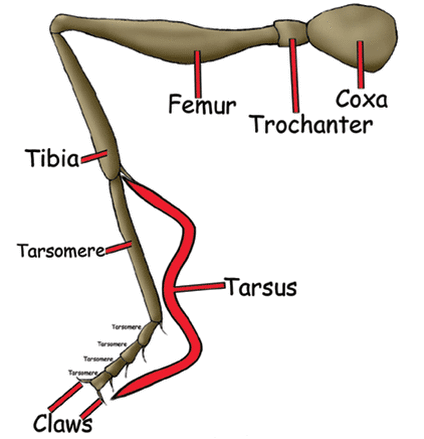
\includegraphics[width=0.2\textwidth]{leg.png}}
    \caption{Leg composition}
    \label{fig8}
\end{figure}

The typical insect leg consists of several segments that are highly adapted to allow the leg to be suitable for its specific requirements. As Figure \ref{fig8} shows, the main segments of the leg are the coxa, trochanter, femur, tibia and tarsus, some of which are not unlike the human leg.\cite{b1} The leg segments have internal muscles, surrounded by tubular structures with articulations for joints. Insect legs are covered in sensilla, sensory organs protruding from the cuticle, that help the insect touch and taste the surface its walking on, as well as proprioceptors for ‘awareness of self’.\cite{b2}

Insect legs are hugely diverse, with different groups of insects bearing very different types of legs that are adapted for their lifestyles.Ambulatory legs are used for walking, for example in beetles (Coleoptera), and bugs (Hemiptera), and are known as the basic, general insect legs (Figure \ref{fig9} left)\cite{b3}. Cursorial legs are modified for running, for example in cockroaches (Blattodea), with long, thin segments (Figure \ref{fig9} right)\cite{b3}.

\begin{figure}
    \centering
    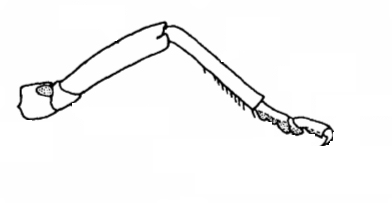
\includegraphics[scale=0.36,align=t]{leg1.png}
    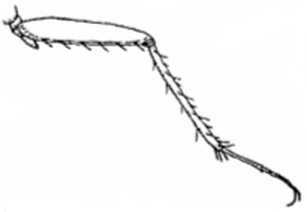
\includegraphics[scale=0.35,align=t]{leg2.jpg}
    \caption{Ambulatory legs and cursorial legs}
    \label{fig9}
\end{figure}




\subsection{Bio-insipred Gait Analysis}\label{ss}
\begin{figure}
    \centerline{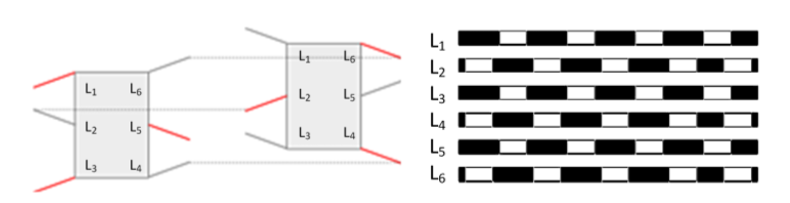
\includegraphics[width=0.4\textwidth]{tri.png}}
    \caption{Tripod gait}
    \label{fig6}
\end{figure}

\begin{figure}
    \centerline{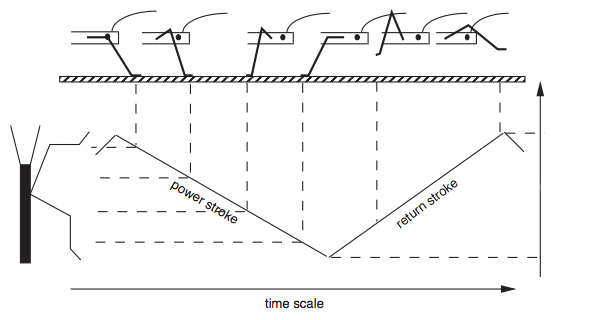
\includegraphics[width=0.4\textwidth]{gait.png}}
    \caption{Gait analysis}
    \label{fig7}
\end{figure}

As Figure \ref{fig6} and Figure \ref{fig7} show, the tripod gait in insects involves three legs protracting (moving in a forward direction from the body), the same three legs exhibiting the power stroke (when the leg is on the ground, supporting the body, and from which it propels the body), followed by those three legs retracting (moving in a backwards direction from the body). As those three legs exhibit the power stoke, the other three legs are protracting. When the power stroke is complete and retraction is occurring, the other three legs are beginning the next power stroke. It is at this time that the three legs to begin motion begin the return stroke in preparation for the next power stroke.\cite{b4}

During tripod gait, three legs move at a time while the other three remain stationary. In contrast to wheeled or tracked locomotion in robots, those with legs are able to operate on irregular and coarse terrain much more readily. They can alter various stages and aspects of their gaits in order to compensate for uneven terrain, including gait patterns and also footholds. However, the risk of slippage upon a extremely smooth surface requires legged robots to have methods of detection and correction in such events. If just one leg slips, it can affect the whole robot’s locomotion and require corrections in the whole gait and thus each leg.\cite{b5}

\section{Design of the Hexapod robot}\label{s3}

\begin{figure}
    \centerline{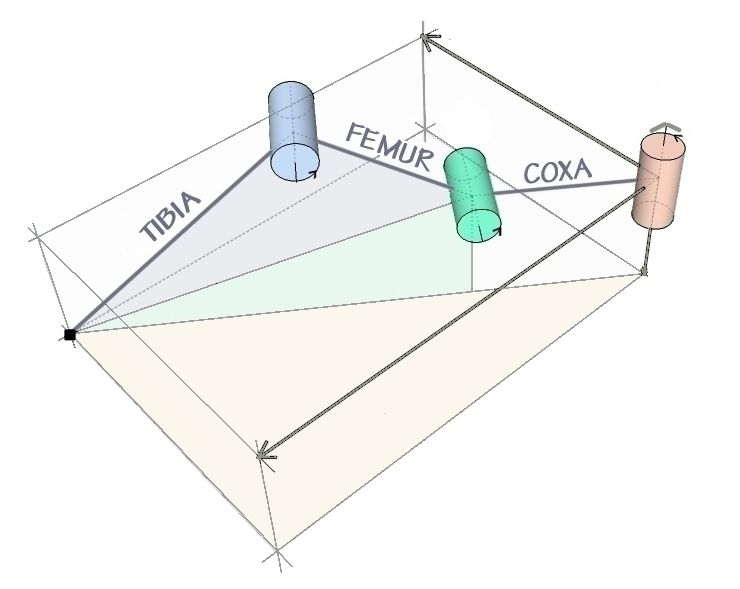
\includegraphics[width=0.35\textwidth]{single_leg.jpg}}
    \caption{Leg model}
    \label{fig2}
\end{figure}

For a single leg, we simplify the leg components of a biological insects' leg, only keeping coxa, femur and tibia as Figure \ref{fig2} shows. Note that the first joint that connects body and coxa is placed vertically. The other two joints are placed horizontally. All the six legs are having the same structure. For the length of each links, we design a length of \(0.08m, 0.10m, 0.16m\) for coxa, femur and tibia respectively. Their weights are \(0.7kg, 0.4kg, 0.6kg\) respectively.

For the body, we use a box with a size of \(0.28m * 0.14m *0.04m\), of which the weight is \(10kg\). Six legs are fixed by joints at the position, of which the distance to edges is \(0.01m\), through symmetrical distribution. The assembled hexapod model is shown in Figure \ref{fig10}. 

\begin{figure}
    \centerline{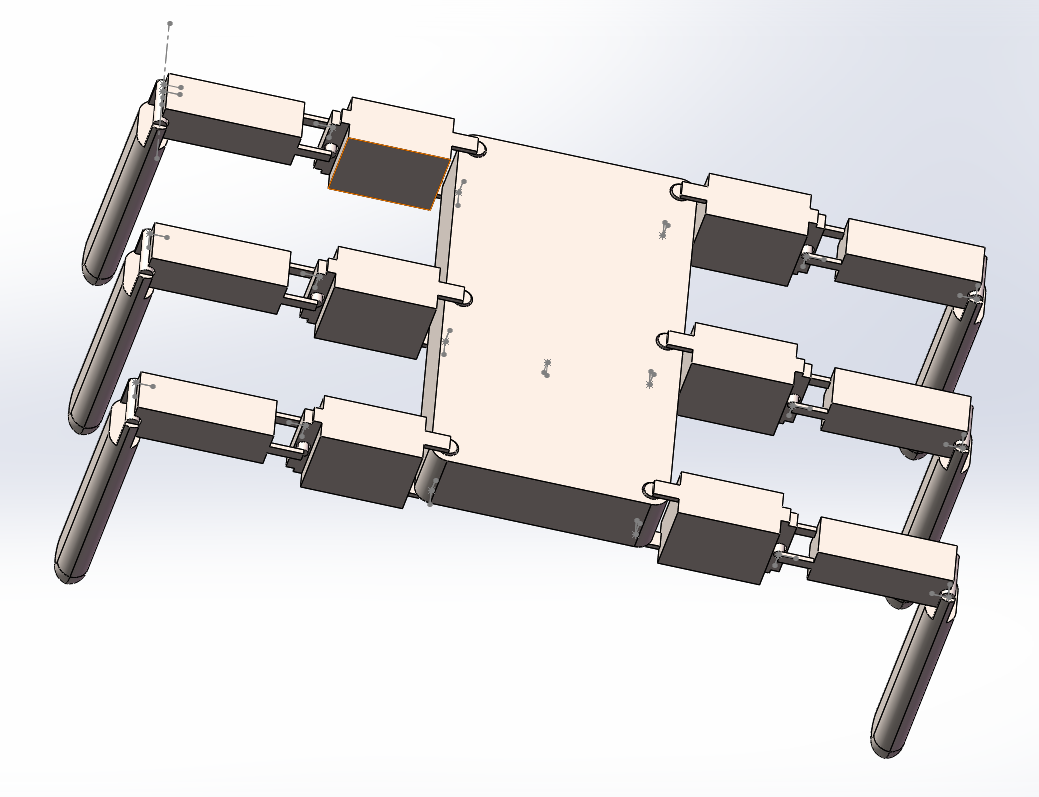
\includegraphics[width=0.4\textwidth]{hexapod.png}}
    \caption{Hexapod model}
    \label{fig10}
\end{figure}

\section{Locomotion Controller Design}\label{s4}

The overall structure of locomotion controller is shown in Figure \ref{fig4}. There are two types of commands, one is to control the posture of the hexapod body, the other one is to control the locomotion. With preset gaits, we can generate foot trajectory based on different methods and parameters. Combined with the desired body posture, whole body inverse kinematics model can be solve to calculate legs vectors, which will be passed to slove leg inverse kinematics to calculate 18 joints angles.

\begin{figure}
    \centerline{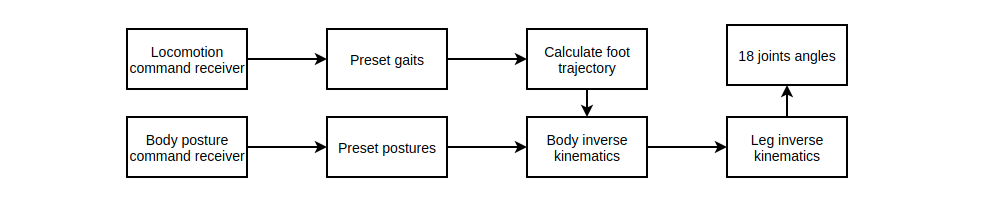
\includegraphics[scale = 0.3]{framework.png}}
    \caption{Overall framework}
    \label{fig4}
\end{figure}

\subsection{Body Inverse Kinematics Model}
\begin{figure}
    \centerline{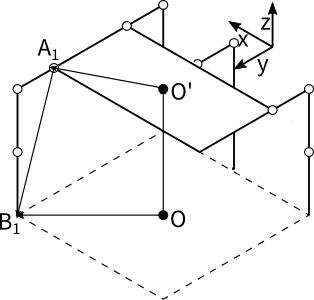
\includegraphics{body_IK.png}}
    \caption{Body inverse kinematics}
    \label{fig1}
\end{figure}
In order to solve each leg's configuration given a desired body posture, we build body inverse kinematics model as Figure \ref{fig1} shows. \textit{O} is the origin of world coordinate and it is also the projection of \textit{O'}, which is the mass center of body. \textit{A$_{1}$} is the coordinate of joint that links leg1 and body. \textit{B$_{1}$} is the coordinate of foot of leg1. The sinlge leg configuration vector can be obtained by 

\begin{equation}\label{1}
    \overrightarrow{A_nB_n}= -\overrightarrow{OO'} - R \cdot \overrightarrow{O'A_n} + \overrightarrow{OB_n} \ \ n=1,...,6
\end{equation}
    
We represent the body posture by kinematics matrix 
\begin{equation}\label{3}
    P = \begin{Bmatrix}
           R & \begin{matrix}
                p_x \\ p_y \\ p_z
                \end{matrix} \\
        \begin{matrix}
        0 & 0 & 0 
        \end{matrix} & 1
        
    \end{Bmatrix}
\end{equation}
where \begin{equation} (p_x, p_y, p_z)^T = \overrightarrow{OO'}\end{equation}

and \textit{R} is the robot body rotation matrix 
\begin{equation}\label{4}
\begin{aligned}
R &= rotx(R)\cdot roty(P) \cdot rotz(Y)\\
&= \begin{bmatrix}
    1 & 0 & 0 \\
    0 & cR & -sR\\
    0 & sR & cR
    \end{bmatrix}
    \begin{bmatrix}
        cP & 0 & sP \\
        0 & 1 & 0\\
        -sP & 0 & cP
        \end{bmatrix}
        \begin{bmatrix}
            cY & -sY & 0 \\
            sY & cY & 0\\
            0 & 0 & 1
            \end{bmatrix}
\end{aligned}
\end{equation}

After obtianing \(\overrightarrow{OB_n}\) based on the design of six foot location, substitute equation (\ref{3})(\ref{4}) into equation (\ref{1}), the single leg configuration vector can be calculated.

\subsection{Single Leg Inverse Kinematics Model}

\begin{figure}
    \centering
    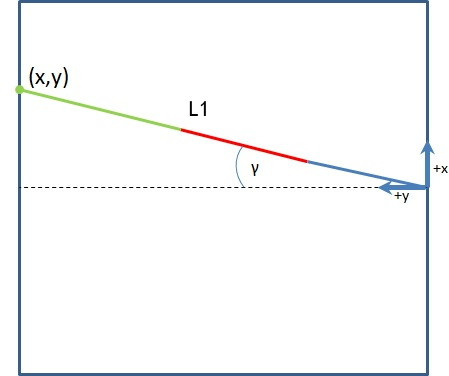
\includegraphics[scale=0.36,align=t]{1-IK-top.jpg}
    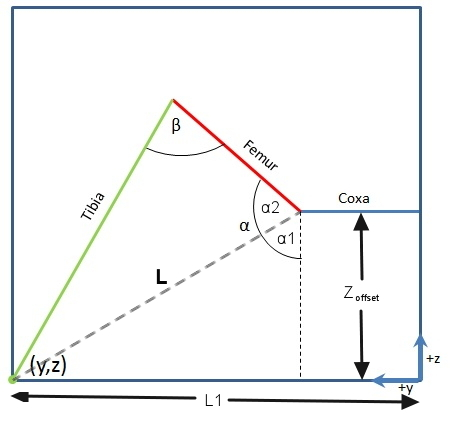
\includegraphics[scale=0.35,align=t]{2-IK-side1.jpg}
    \caption{Top view and side view}
    \label{fig3}
\end{figure}

 To get joint angles, we are going to solve the single leg kinematics model, which is shown in Figure \ref{fig2}. To better illustrate the calculation process, Figure \ref{fig3} shows the top view and side view of the model.

Note that we have already obtained the leg vector, so the foot point coordinate \textit{(x,y,z)} is given. From top view, it is straightforward that \(\gamma\) can be calculated by 
\begin{equation}
    \gamma = tan^{-1} \frac{x}{y}
\end{equation}

From the side view, we will split \(\alpha\) into \(\alpha_1\) and \(\alpha_2\). We can get \(\alpha_1\) by working out \textit{L} first.

\begin{equation}
    L=\sqrt{Z^{2}_{offset} + (L_1 - L_{coxa})^2}
\end{equation}
\begin{equation}
    \alpha_1 = cos^{-1}(\frac{Z_{offset}}{L})
\end{equation}

In our case, here \(Z^{2}_{offset}=z\). With the help of Cosine Rules,

\begin{equation}
    \alpha_2 = cos^{-1}(\frac{L_{tibia}^2-L_{femur}^2 - L^2}{-2\cdot L \cdot L_{femur}})
\end{equation}

\begin{equation}
    \beta = cos^{-1}(\frac{ L^2-L_{tibia}^2-L_{femur}^2}{-2\cdot L_{tibia} \cdot L_{femur}})
\end{equation}

Then, \(\alpha\) can be calculated by 
\begin{equation}
    \begin{aligned}
        \alpha &= \alpha_1 + \alpha_2\\
        &= cos^{-1}(\frac{Z_{offset}}{L})+cos^{-1}(\frac{L_{tibia}^2-L_{femur}^2 - L^2}{-2\cdot L \cdot L_{femur}})
    \end{aligned}
\end{equation}

As the design of six legs are similar, the solution introduced above can be applied to all six legs. Hence, all the 18 joints angles can be calculated.

\subsection{Single Foot Trajectory Design}

To generate a single foot trajectory, we introduce a parameter \(s\) to determine the number of intermedia points between two foot steps. We also want to control the step size \(L\) and step height \(H\), hence we introduce a modified cycloid function on \(X-Z\) projection plane for forward half step (green arrows), which is return stroke as Section \ref{ss} introduced. On \(Y\)axis, all the points are set to average distribution considering the less motion on this axis. Given start foot point coordinate of a step \((x_s, y_s, z_s)\) and end foot point coordinate \((x_e, y_e, z_e)\), the trajectory containing \(n\) intermedia points can be dirived by 

\begin{figure}
    \centerline{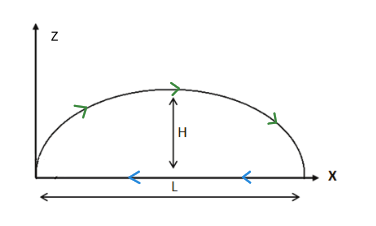
\includegraphics[width=0.4\textwidth]{traj.png}}
    \caption{cycloid function}
    \label{fig5}
\end{figure}

\begin{equation}
    \begin{cases}
    t_n &= n \cdot \frac{2\pi}{s}\\
    x_n &= x_s+\frac{L}{2\pi} \cdot(t_n- sin(t_n))\\
    z_n &= z_s+\frac{H}{2}\cdot(1- cos(t_n))\\
    y_n &= y_s + (y_e - y_s)\cdot \frac{n}{s}    
    \end{cases}
\end{equation}

For the backward half step (blue arrows), which is power stroke as described in Section \ref{ss}, as the leg need to make use of the friction between foot and ground to act force in joints, we adopt average distribution for intermedia points on \(X-Y\) plane to keep foot always contact with ground. 

Till now, a whole step foot trajectory has been generated. The generation process can be implement in all six legs.

\subsection{Gait Design}

For gait design, we completely follow the result of gait analysis from biology, which is described in Section \ref{ss}. The straightforward illusration can be found in Figure \ref{fig6}. To avoid repetation, we will not described again here.

Details of the design is described as follow, we set step size to be \(0.08m\) and step height to be \(0.04m\). For smooth factor we choose \(s=4\) to get smooth trajectory without consuming too much computational resource.

\section{Simulation Experiments}\label{s5}
The simulation envirnment are built based on Robot Operating System (ROS) and a physical engine Gazebo.

\begin{figure}
    \centerline{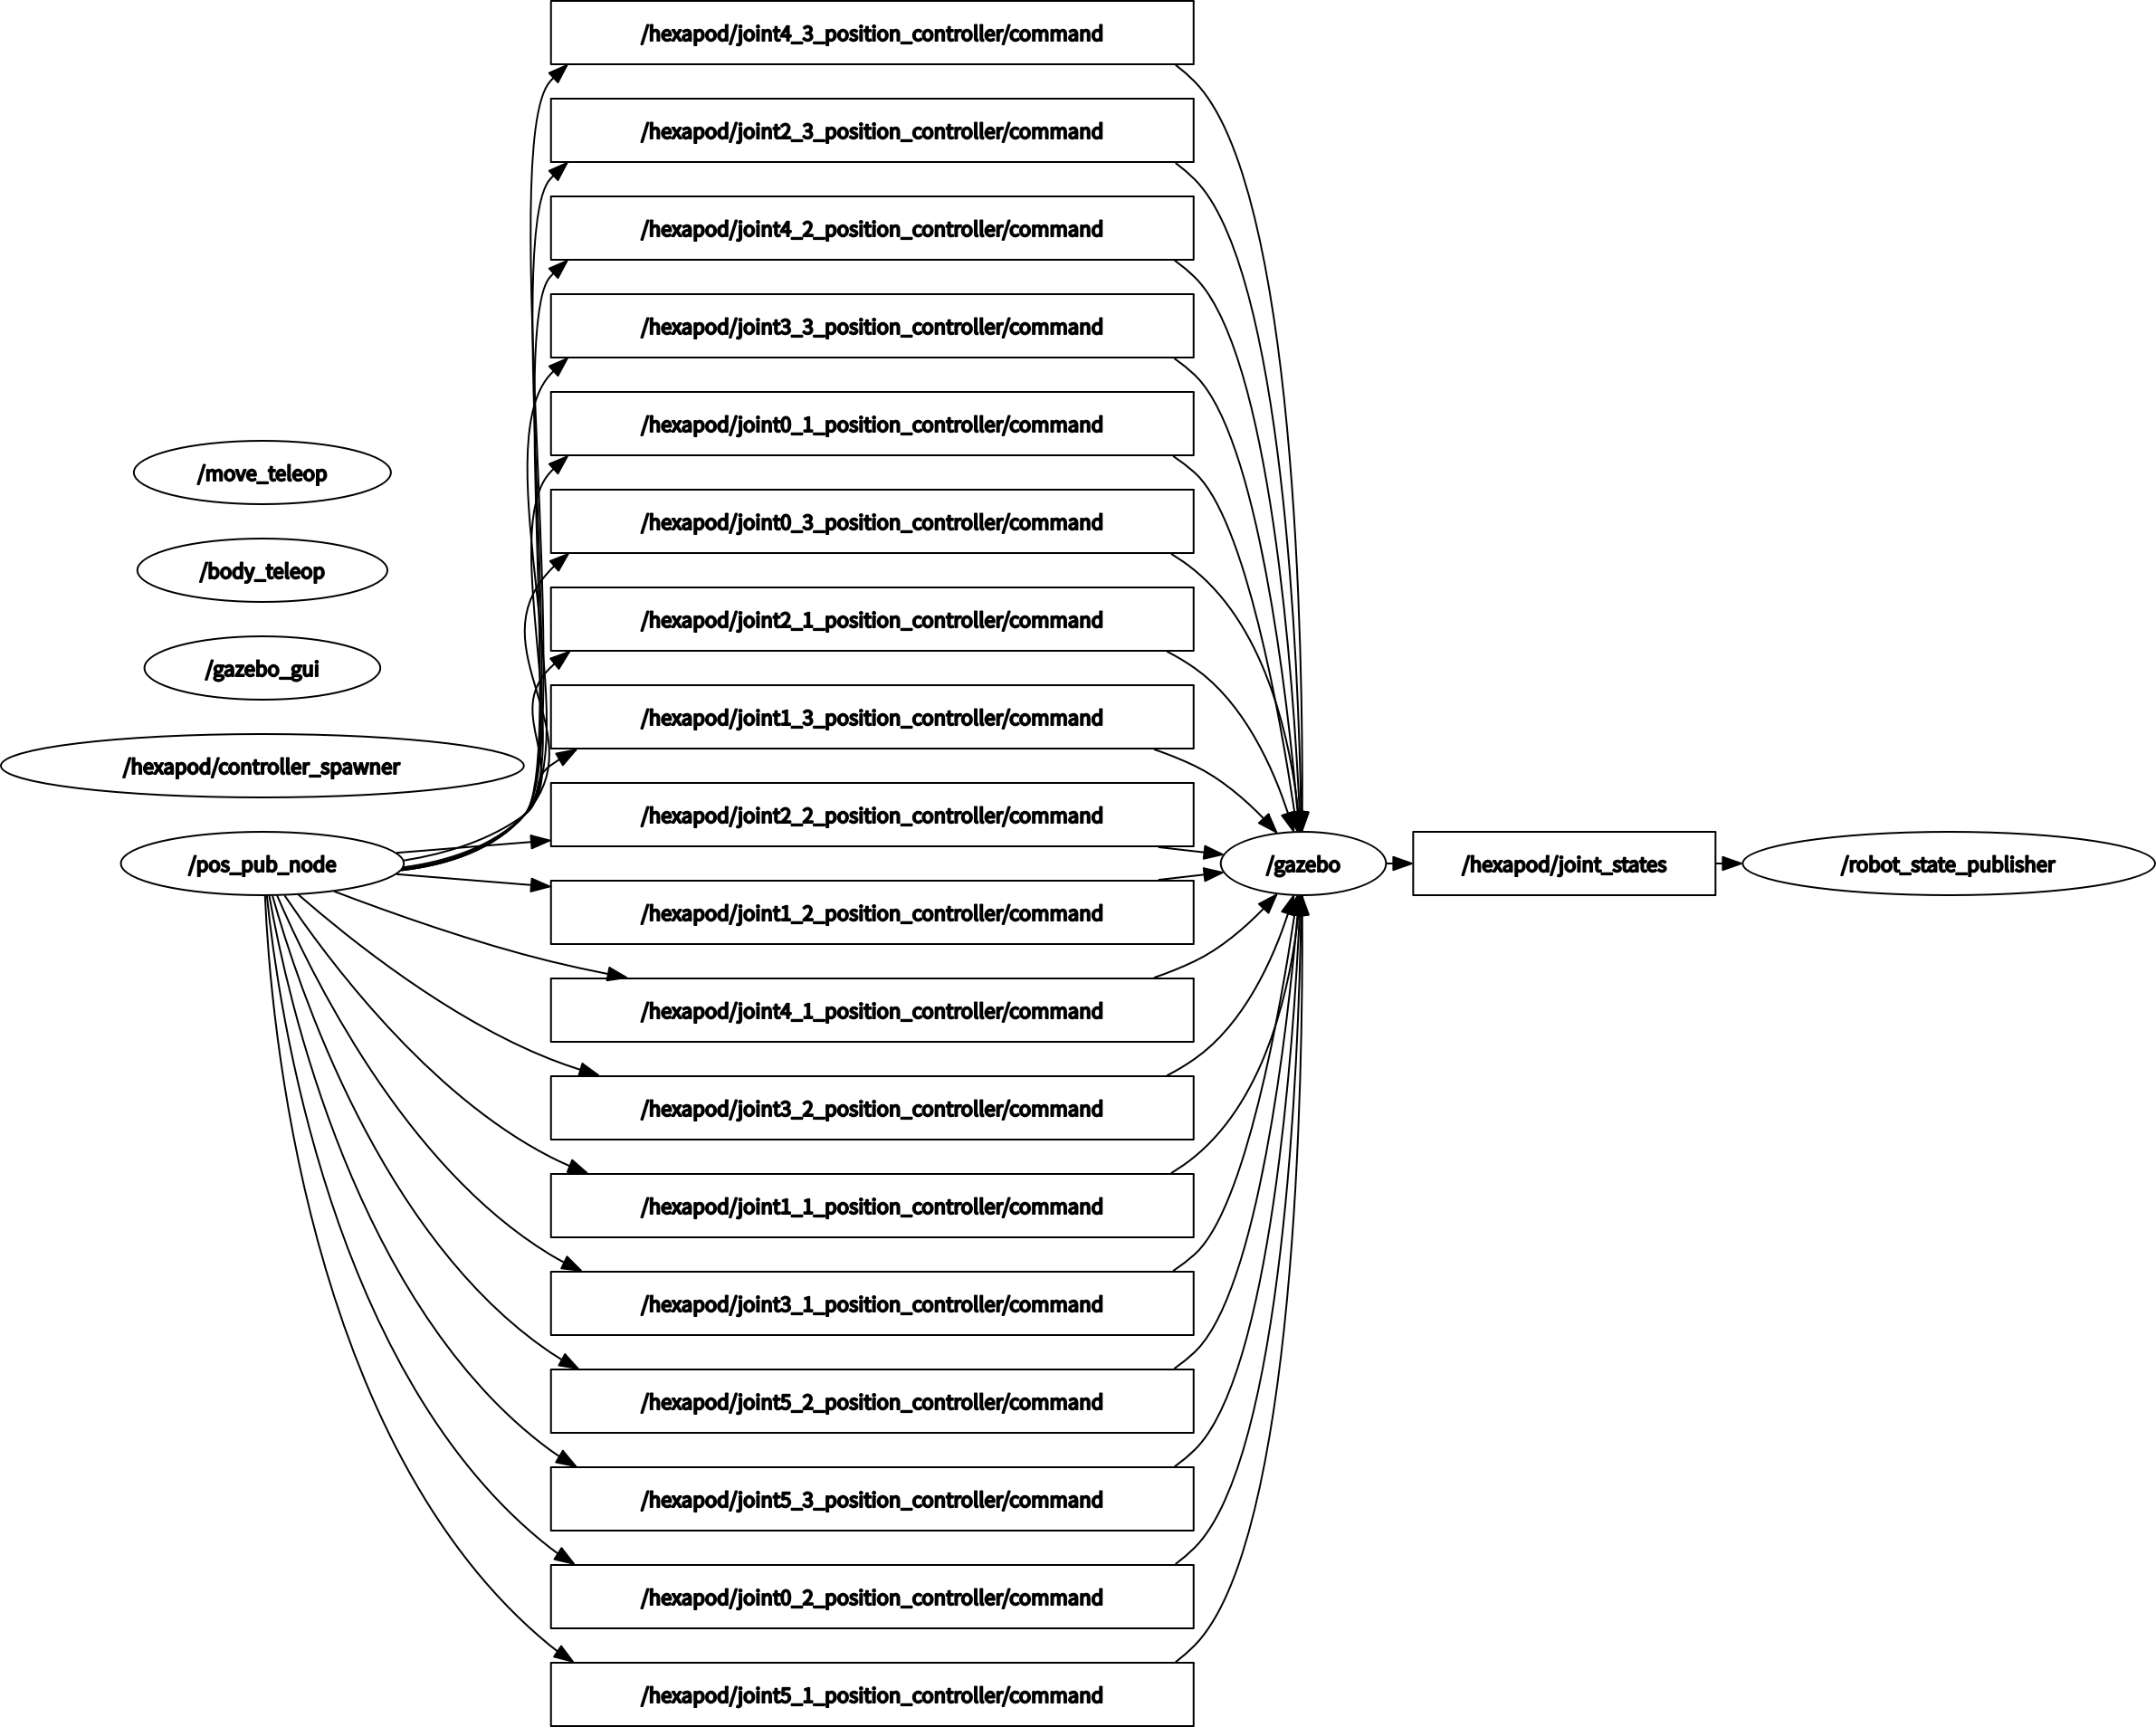
\includegraphics[width=0.5\textwidth]{rosgraph.png}}
    \caption{ROS framework}
    \label{fig11}
\end{figure}

\subsection{Overall Framework}
ROS mostly takes the advantages of node publish/subscribe, serivice and parameter server mechanism, which is easy to handle complex robot system. The overall framework in our project is shown in Figure \ref{fig11}. Node \(</move\_teleop>\) and node \(</body\_teleop>\) are used to choose preset gait and body posture by changing the parameters in parameter server. Node \(</gazebo\_gui>\) and node \(</hexapod/controller\_spawner>\) and are uesd to initialize the simulation system. After calculating the desired 18 joints angles, we use node \(</pos\_pub\_node>\) to publish each angel to corresponding topics. Then the controllers for the joints subscribe data from corresponding topics and actuate joints in simulation environment through node \(</gazebo>\).
\subsection{Setting Details}

For each joint, we are using \(ros\_control\) plugins for actuation. The type of controller using for each joint is \(effort\_controllers/JointPositionController\) with hardware interface \(/EffortJointInterface\). After tuned, PID gains are set to \(k_p = 50, k_i = 0.01, k_d=1\) in order to achieve good performance. The publish rate of controllers is set to \(300\).  

For the Gazebo contact surface friction coefficients, we use default parameters, which is \(\mu_1 = \mu _2 = 1.0\).

\subsection{Body Posture Control}

The posture control experiment results are shown in Figure \ref{fig111}, \((a)\) is the default posture, \((b-h)\) are different preset postures.

\begin{figure}
    \centering
    \subfigure[Default posture]{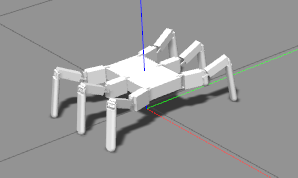
\includegraphics[scale = 0.4]{b1.png}} 
    \subfigure[\(p_y -0.03\)]{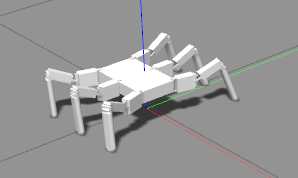
\includegraphics[scale = 0.4]{b11.png}} \\
    \subfigure[\(p_y +0.03\)]{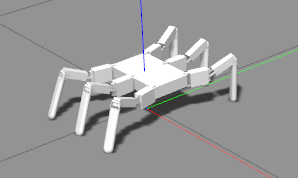
\includegraphics[scale = 0.4]{b2.png}} 
    \subfigure[\(p_x +0.05\)]{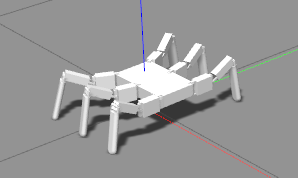
\includegraphics[scale = 0.4]{b3.png}} \\
    \subfigure[\(p_x - 0.05\)]{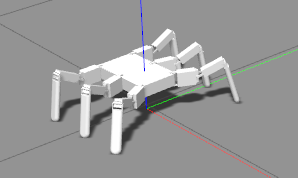
\includegraphics[scale = 0.4]{b4.png}} 
    \subfigure[\(Pitch - 10^o\)]{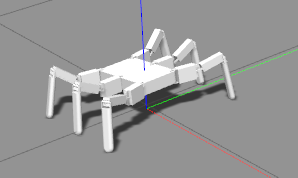
\includegraphics[scale = 0.4]{b5.png}} \\
    \subfigure[\(Pitch + 10^o\)]{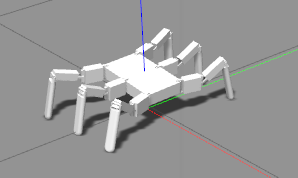
\includegraphics[scale = 0.4]{b6.png}}  
    \subfigure[\(p_z-0.02\)]{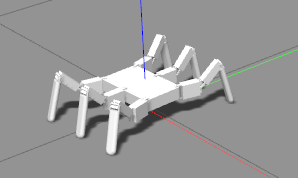
\includegraphics[scale = 0.4]{b9.png}} \\
    \caption{Body posture control}
      \label{fig111}
\end{figure}

\subsection{Locomotion}
The locomotion experiments results are presented in Figure \ref{fig1111}, in which \((a)\) is the start point, \((b)\) is captured during forward gait while \((c)\) is captured during backward gait. Note the simulation time at the bottom of above mentioned figure can prove the locomotion is successful. Meanwhile, due to our design framework, the hexapod robot can change to arbitrary preset posture at any time during the locomotion. \ref{fig1111} \((d)\) shows an example that the hexapod robot is moving forward with a posture of \(Pitch - 10^o\).
\begin{figure}
    \centering
    \subfigure[Start point]{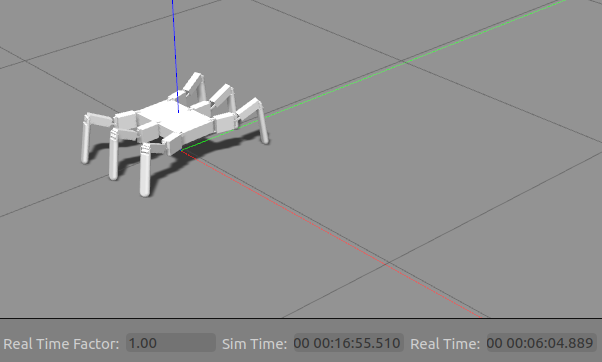
\includegraphics[scale= 0.2]{a0.png}}
    \centering
    \subfigure[Forward gait]{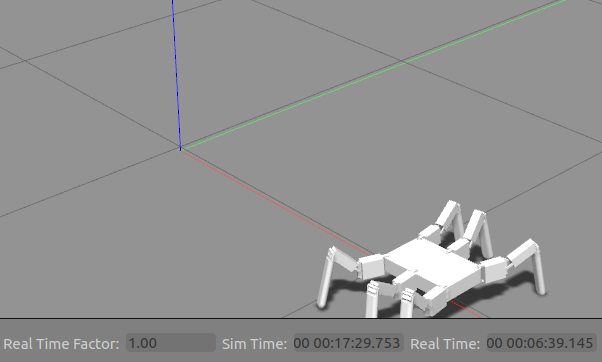
\includegraphics[scale= 0.2]{a2.png}}\\
    \subfigure[Backward gait]{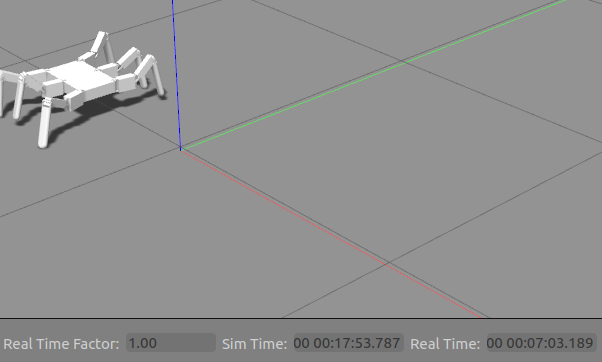
\includegraphics[scale= 0.2]{a1.png}}
    \centering
    \subfigure[Forward gait \((Pitch - 10^o)\)]{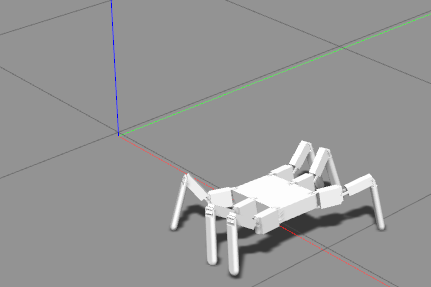
\includegraphics[scale= 0.25]{a3.png}}
    \caption{Hexapod locomotion}
    \label{fig1111}
\end{figure}

\section{Conclusion}

In this project, we get inspiration from biology animals and build a hexapod robot model. After analysing insects gait, we implement it to our hexapod robot by buiding and solving body inverse kinematics and leg inverse kinematics. Then we build a efficent control framework based on ROS and Gazebo to do experiments in simulation environment. Our proposed method is successful for controlling hexapod robot posture and locomotion. Our proposed contorl framework is efficent that the hexapod robot can change body postures at arbitrary time during locomotion.

\begin{thebibliography}{00}   

    \bibitem{a2}
    Manuel F. Silva, J. A. Tenreiro Machado, (2006), A Historical Perspective of Legged Robots, Journal of Vibration and Control 2007 13: 1447,
    DOI: 10.1177/1077546307078276.
    \bibitem{a3}
    Joaquin Estremera and Pablo Gonzales de Santos, (2005), Generating Continuous Free Crab Gaits for Quadruped Robots on Irregular Terrain, IEEE Transactions on Robotics, Vol. 21, No. 6. December.
    \bibitem{a15}
    J. P. Flores Fernandes, J. C. Pimenta Claro, Fernando Ribeiro. Design of a Hexapod Robotic System.    
    \bibitem{aa}
    García-López, M., Gorrostieta-Hurtado, E., Vargas-Soto, E., Ramos-Arreguín, J., Sotomayor-Olmedo, A., \& Morales, J. M. (2012). Kinematic analysis for trajectory generation in one leg of a hexapod robot. Procedia Technology, 3, 342-350.
    \bibitem{a16}
    Jing Liu, Min Tan and Xiaoguang Zhao, (2007), Legged robots – an overview, Transactions of the Institute of Measurement and Control 2007 29: 185, DOI: 10.1177/0142331207075610.
    \bibitem{b1} Delcomyn, F., Nelson, M.E. (2000). Architectures for a biomimetic hexapod robot. Robotics and autonomous systems 30:5-15.
    \bibitem{b2}
    Steinbrecht, R.A. (1996). The structure and function of insect olfactory sensilla. Ciba foundation symposium 200: 158-174.
    \bibitem{b3}
    Hoffman, M.P., Frodsham, A.C. (1993). Natural enemies of vegetable insect pests. Cooperative extension 63.
    
    \bibitem{b4}
    Ferrell, C. (1995). A Comparison of Three Insect Inspired Locomotion Controllers, Robotics and autonomous systems 16.2, 135-159.
    \bibitem{b5}
    Hörger, Marcus, Kottege, N., Bandyopadhyay, T., Elfes, A., and Moghadam, P. Real-Time Stabilisation for Hexapod Robots, Autonomous Systems, CSIRO Computational Informatics, Queensland Center for Advanced Technology, Brisbane, QLD.
\end{thebibliography}

\end{document}